\documentclass{beamer}
\usepackage[T1]{fontenc}
\usepackage[utf8]{inputenc}
\usepackage{lmodern}
\usepackage[polish]{babel}
\usepackage{graphicx}

\usetheme{AGH}

\title[Interpolacja barwna obrazu]{Równoległa interpolacja obrazu barwnego
  z~kamery cyfrowej}

\author[B. Bułat, T. Drzewiecki]{Bartłomiej Bułat, Tomasz Drzewiecki}

\date[2011]{24.01.2012}

\institute[AGH]
{Wydział EAIiIB\\ 
Katedra Automatyki i Inżynierii Biomedycznej
}

\setbeamertemplate{itemize item}{$\maltese$}

\begin{document}

{
\usebackgroundtemplate{
\includegraphics[width=\paperwidth]{titlepagepl}} % wersja polska
 \begin{frame}
   \titlepage
 \end{frame}
}

%---------------------------------------------------------------------------

%% Figure example
%\begin{figure}
%  \includegraphics[width=0.5\textwidth]{filename}
%  \caption{Figure caption}
%  \label{fig:label}
%\end{figure}

\begin{frame}
\frametitle{Plan prezentacji}
	
  \begin{itemize}
  	\item Cele projektu
	  \item Wstęp teoretyczny
  	\item Programowanie OpenCL
  	%TODO: @Tomek, dopisz swoje
  	\item Podsumowanie
	\end{itemize}

\end{frame}

\begin{frame}
	\frametitle{Cele projektu}
	
  Celem projektu była implementacja algorytmu interpolacji barwnej obrazu z kamery
  z użyciem zrównoleglania obliczeń na karcie graficznej (OpenCL). 
  
  Wynikiem prac miała być
  biblioteka realizująca wymieniony algorytm, biblioteka obsługująca kamerę wysokiej rozdzielczości
  oraz aplikacja integrująca obie biblioteki pozwalająca na przetwarzanie obrazu z kamery w czasie 
  rzeczywistym.  
\end{frame}

\begin{frame}
  \frametitle{Matryca Bayer-a}
  
  \begin{columns}
  \begin{column}{5cm}
  Kamery używają pewnej topologii filtrów kolorowych na matrycy. Matryca Bayer-a to topologia odzwiercielająca
  sposób postrzegania kolorów przez ludzkie oko. Na rysynku obok pokazano powiekszony układ
  filtów na tej matrycy.
  \end{column}
  \begin{column}{5cm}
    \begin{center}
    \begin{figure}

	  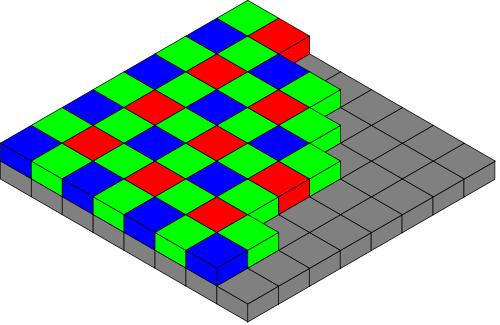
\includegraphics[width=\textwidth]{bayer_pattern_sensor}
	  \caption{Układ filtrów kolorowych na matrycy Bayer-a}
	  \label{fig:pattern}
    \end{figure}
    \end{center}
	\end{column}
	\end{columns}
	
\end{frame}

\begin{frame}
	\frametitle{Interpolacja barwna}
	
	\begin{columns}
	\begin{column}{4cm}
    \begin{center}
    \begin{figure}

	  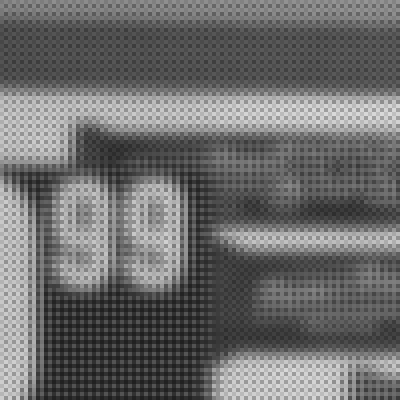
\includegraphics[width=\textwidth]{raw_image}
	  \caption{Surowy obraz z matrycy Bayer-a}
	  \label{fig:raw_image}
    \end{figure}
    \end{center}
  \end{column}
  \begin{column}{6cm}
	Na rysunku obok przedstawiony jest powiekszony fragment obrazu surowego, odczytanego prosto z matrycy.
	Aby przekształcić taki obraz w obraz kolorowy, należy dla każdego piksela interpolować wartość kolorów:
	{\color{red}czerwonego}, {\color{green}zielonego} oraz {\color{blue}niebieskiego}.
	
	Interpolacja wykonywana jest z wykorzystaniem wartości pikseli sąsiednich.
  \end{column}
  \end{columns}
\end{frame}

\begin{frame}
  \frametitle{Podsumowanie}
  
\end{frame}

\end{document}

